\documentclass[tikz,border=12pt]{standalone}
\usepackage[T1]{fontenc}
\usepackage{mathpazo}
\usepackage{amsmath,amssymb}
\usetikzlibrary{arrows.meta, calc}

\definecolor{stblue}{HTML}{7B97AD}
\definecolor{rwgold}{HTML}{B8995E}
\definecolor{sage}{HTML}{7A9A7E}
\definecolor{dkbrown}{HTML}{3D3530}
\definecolor{wmgray}{HTML}{7B7067}
\definecolor{cream}{HTML}{F9F6F0}
\definecolor{border}{HTML}{D4C9B8}
\definecolor{terracotta}{HTML}{C47A6A}
\definecolor{lavender}{HTML}{907EA0}

\begin{document}
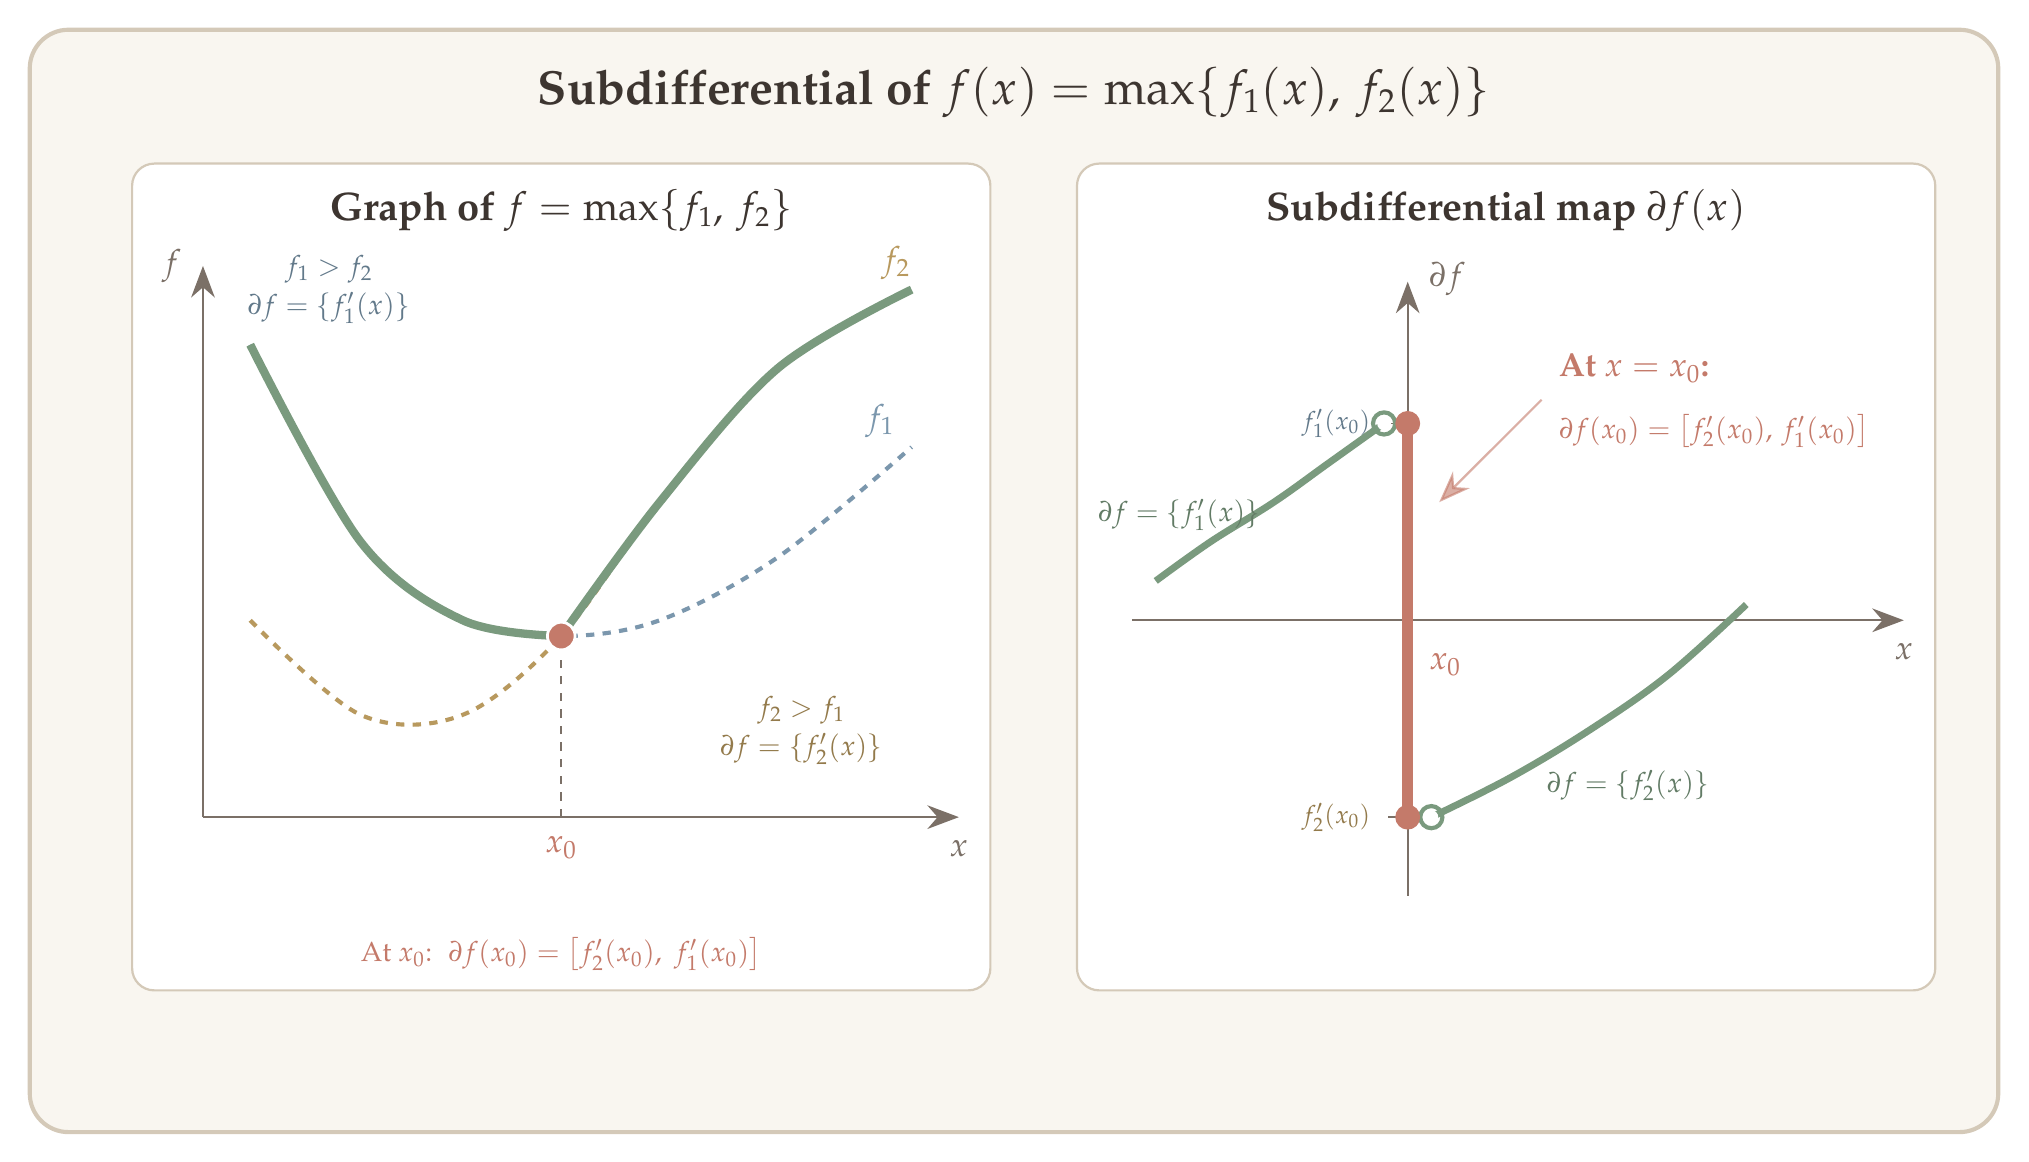
\begin{tikzpicture}[>={Stealth[length=4mm, width=3mm]}]

% Background
\fill[cream, rounded corners=14pt] (-1.0,-1.5) rectangle (24.0,12.5);
\draw[border, line width=1.5pt, rounded corners=14pt] (-1.0,-1.5) rectangle (24.0,12.5);

% Title
\node[text=dkbrown, font=\LARGE\bfseries] at (11.5,11.7)
  {Subdifferential of $f(x) = \max\{f_1(x),\, f_2(x)\}$};

% ============================================================
% Left panel: graph of max{f1, f2}
% ============================================================
\fill[white, rounded corners=8pt] (0.3,0.3) rectangle (11.2,10.8);
\draw[border, line width=0.8pt, rounded corners=8pt] (0.3,0.3) rectangle (11.2,10.8);
\node[text=dkbrown, font=\Large\bfseries] at (5.75,10.2)
  {Graph of $f = \max\{f_1,\, f_2\}$};

% Axes — origin at bottom-left
\draw[wmgray, line width=0.8pt, ->] (1.2,2.5) -- (10.8,2.5);
\draw[wmgray, line width=0.8pt, ->] (1.2,2.5) -- (1.2,9.5);
\node[text=wmgray, font=\large] at (10.8,2.1) {$x$};
\node[text=wmgray, font=\large] at (0.8,9.5) {$f$};

% f1(x) — dashed stblue: convex, higher on left, descends to crossing, rises gently right
\draw[stblue, line width=1.5pt, dashed]
  plot[smooth, tension=0.55] coordinates
  {(1.8,8.5) (3.2,6.0) (4.5,5.0) (5.75,4.8) (7.0,5.0) (8.5,5.8) (10.2,7.2)};

% f2(x) — dashed rwgold: convex, lower on left, rises steeply to right
\draw[rwgold, line width=1.5pt, dashed]
  plot[smooth, tension=0.55] coordinates
  {(1.8,5.0) (3.2,3.8) (4.5,3.8) (5.75,4.8) (7.0,6.5) (8.5,8.2) (10.2,9.2)};

% Max function — thick sage, follows f1 on left then f2 on right
\draw[sage, line width=3pt]
  plot[smooth, tension=0.55] coordinates
  {(1.8,8.5) (3.2,6.0) (4.5,5.0) (5.75,4.8)};
\draw[sage, line width=3pt]
  plot[smooth, tension=0.55] coordinates
  {(5.75,4.8) (7.0,6.5) (8.5,8.2) (10.2,9.2)};

% Crossing point
\fill[terracotta] (5.75,4.8) circle (5pt);
\draw[white, line width=1pt] (5.75,4.8) circle (5pt);

% x0 label and vertical dashed line to axis
\draw[wmgray, line width=0.6pt, dashed] (5.75,2.5) -- (5.75,4.5);
\node[text=terracotta, font=\large\bfseries, below=2pt] at (5.75,2.45) {$x_0$};

% f1, f2 curve labels — near curve ends
\node[text=stblue, font=\large\bfseries, anchor=south] at (9.8,7.2) {$f_1$};
\node[text=rwgold, font=\large\bfseries, anchor=south] at (10.0,9.2) {$f_2$};

% Region labels — placed in open areas
\node[text=stblue!80!black, font=\normalsize, align=center] at (2.8,9.2)
  {$f_1 > f_2$\\[2pt]$\partial f = \{f_1'(x)\}$};
\node[text=rwgold!80!black, font=\normalsize, align=center] at (8.8,3.6)
  {$f_2 > f_1$\\[2pt]$\partial f = \{f_2'(x)\}$};

% Annotation at bottom of panel
\node[text=terracotta, font=\normalsize, align=center, anchor=north] at (5.75,1.1)
  {At $x_0$:\; $\partial f(x_0) = \bigl[f_2'(x_0),\; f_1'(x_0)\bigr]$};

% ============================================================
% Right panel: subdifferential map (set-valued)
% ============================================================
\fill[white, rounded corners=8pt] (12.3,0.3) rectangle (23.2,10.8);
\draw[border, line width=0.8pt, rounded corners=8pt] (12.3,0.3) rectangle (23.2,10.8);
\node[text=dkbrown, font=\Large\bfseries] at (17.75,10.2)
  {Subdifferential map $\partial f(x)$};

% Axes — vertical axis at x=16.5 to give more room on right
% Horizontal axis at y=5.0
\draw[wmgray, line width=0.8pt, ->] (13.0,5.0) -- (22.8,5.0);
\draw[wmgray, line width=0.8pt, ->] (16.5,1.5) -- (16.5,9.3);
\node[text=wmgray, font=\large] at (22.8,4.6) {$x$};
\node[text=wmgray, font=\large, anchor=south west] at (16.65,9.0) {$\partial f$};

% x0 tick on horizontal axis — label offset to the right so it doesn't sit under the bar
\draw[terracotta, line width=0.8pt] (16.5,4.8) -- (16.5,5.2);
\node[text=terracotta, font=\large\bfseries, anchor=north west] at (16.65,4.7) {$x_0$};

% Tick marks for f1'(x0) and f2'(x0) on vertical axis
% f1'(x0) at y=7.5, f2'(x0) at y=2.5
\draw[wmgray, line width=0.6pt] (16.25,7.5) -- (16.5,7.5);
\node[text=stblue!80!black, font=\small, anchor=east] at (16.15,7.5) {$f_1'(x_0)$};
\draw[wmgray, line width=0.6pt] (16.25,2.5) -- (16.5,2.5);
\node[text=rwgold!80!black, font=\small, anchor=east] at (16.15,2.5) {$f_2'(x_0)$};

% Left branch: derivative of f1 for x < x0 (f1 convex, so f1' increasing)
\draw[sage, line width=2.5pt]
  plot[smooth, tension=0.6] coordinates
  {(13.3,5.5) (14.0,6.0) (14.8,6.5) (15.5,7.0) (16.2,7.5)};
% Open circle at x0 boundary
\draw[sage, line width=1.5pt] (16.2,7.5) circle (4pt);
\fill[white] (16.2,7.5) circle (2.5pt);
% Label above the curve, well left of the tick label
\node[text=sage!80!black, font=\normalsize, above=6pt] at (13.6,5.8)
  {$\partial f = \{f_1'(x)\}$};

% Right branch: derivative of f2 for x > x0 (f2 convex, so f2' increasing)
\draw[sage, line width=2.5pt]
  plot[smooth, tension=0.6] coordinates
  {(16.8,2.5) (17.8,3.0) (18.8,3.6) (19.8,4.3) (20.8,5.2)};
% Open circle at x0 boundary
\draw[sage, line width=1.5pt] (16.8,2.5) circle (4pt);
\fill[white] (16.8,2.5) circle (2.5pt);
% Label below the curve
\node[text=sage!80!black, font=\normalsize, below=5pt] at (19.3,3.4)
  {$\partial f = \{f_2'(x)\}$};

% At x = x0: vertical interval [f2'(x0), f1'(x0)]
\draw[terracotta, line width=4pt, line cap=round] (16.5,2.5) -- (16.5,7.5);
\fill[terracotta] (16.5,2.5) circle (4.5pt);
\fill[terracotta] (16.5,7.5) circle (4.5pt);

% Annotation for x = x0 — placed to the right with room to spare
\node[text=terracotta, font=\large\bfseries, align=left, anchor=west] at (18.3,8.2)
  {At $x = x_0$:};
\node[text=terracotta, font=\normalsize, align=left, anchor=west] at (18.3,7.4)
  {$\partial f(x_0) = \bigl[f_2'(x_0),\, f_1'(x_0)\bigr]$};

% Arrow from annotation to vertical bar
\draw[terracotta, line width=0.8pt, ->, opacity=0.6] (18.2,7.8) -- (16.9,6.5);

\end{tikzpicture}
\end{document}
